\documentclass{beamer}
\usepackage{amsmath}
\usepackage[utf8]{inputenc}
\usepackage{graphicx}
\usetheme{AnnArbor}
\usecolortheme{default}

\title{Exploratory Projection Pursuit}
\subtitle{ EE1390 INTRO TO AI AND ML}
\author{V.L.Narasimha Reddy EE18BTECH11046 \\Aditya Pedavegi EE18BTECH11034 }
\date{March 2019}

\begin{document}
\maketitle
\begin{frame}{INTRODUCTION}
Linear Discriminant Analysis (LDA) is  used for dimensional reduction and data classification of higher dimensional data
\\
The goal is to project a dataset onto a lower-dimensional space with good class-separability.
\\
This is one of the techniques used  in the projection pursuit.
\end{frame}
\begin{frame}{Application}
We have the iris dataset of three different species of leaves of 150 samples of 50 sample each.
\\
The variable matrix is constructed based on four different features.They are
\\
\rightarrow{$sepal length$}
\\
\rightarrow{$sepal width$}
\\
\rightarrow{$petal length$}
\\
\rightarrow{$petal width$}
\end{frame}
\begin{frame}{Data}
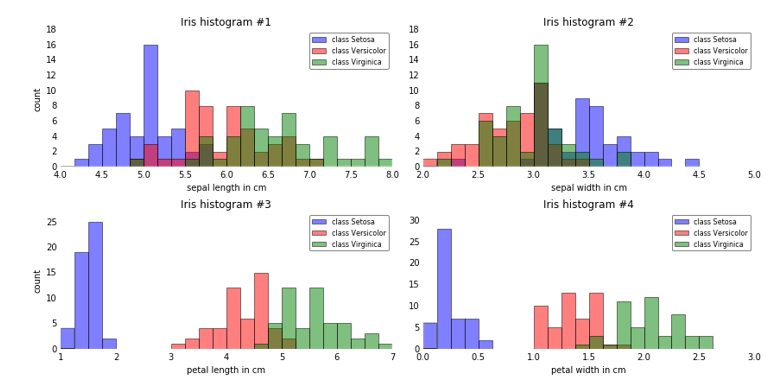
\includegraphics[scale = 0.6]{epp_1.PNG}
    
\end{frame}
\begin{frame}{INDEX}
\rightarrow{$Reading the data set$}
\\
\rightarrow{$Computing the d-dimensional mean vectors$}
\\
\rightarrow{$Computing the scatter matrices$}
\\
\rightarrow{$Computing the eigen values$}
\\
\rightarrow{$Optimization$}
\\
\rightarrow{$Projection onto a new subspace$}


\end{frame}

\begin{frame}{Reading the dataset}
The varaible matrix X is 150 x 4 dimension which reduces to Y which is 150 x 1 dimension.
\begin{equation}
X=
\begin{bmatrix}
x_1_{$sepal length$}  & x_1_{$sepal width$} & x_1_{$petal length$} & x_1_{$petal width$}
\\
x_2_{$sepal length$}  & x_2_{$sepal width$} & x_2_{$petal length$} & x_2_{$petal width$}
\\
....
\\
x_{150}_{$sepal length$}  & x_{150}_{$sepal width$} & x_{150}_{$petal length$} & x_{150}_{$petal width$}
\end{bmatrix}
\end{equation}
\begin{equation}
Y=
\begin{bmatrix}
w_1 & r_1
\\
w_1 & r_1
\\
...
\\
w_2 & r_2
\\
w_2 & r_2
\\
...
\\
w_3 & r_3
\\
w_3 & r_3
\\
...
\end{bmatrix} 
\end{equation}
\end{frame}
\begin{frame}{Computing the d-dimensional mean vectors}
Now we have to compute the mean vectors of three different species
\\
\begin{equation}
m_i=
\begin{bmatrix}
\mu_i_{$sepal length$}
\\
\mu_i_{$sepal width$}
\\
\mu_i_{$petal length$}
\\
\mu_i_{$petal width$}
\end{bmatrix}
\end{equation}
\\
for i= 1,2,3..
\\
Mean Vector class 1: [ 5.006  3.418  1.464  0.244]
\\
Mean Vector class 2: [ 5.936  2.77   4.26   1.326]
\\
Mean Vector class 3: [ 6.588  2.974  5.552  2.026]
\\
overall mean m is computed by
\begin{equation}
    m=(m_1+m_2+m_3)/3.0
\end{equation}
\end{frame}
\begin{frame}{Computing the scatter matrices}
Now we will compute two 4 x 4 dimensional matrices one is within-class scatter matrix and other is between-class scatter matrix.
\\
\\
The within class scatter matrix is
\begin{equation}
    S_W=\sum_{i=1}^{c}{S_i}
\end{equation}

$$    S_i= \sum_{x=1}^{n_i}{(x_i-m_i)(x_i-m_i)^T} $$

\\
where $S_i$ is a scatter matrix of every class and $m_i$ is the mean vector
\\
Now we compute between-class scatter matrix 
\begin{equation}
   S_B=\sum_{i=1}^{c}{N_i(m_i-m)(m_i-m)^T} 
\end{equation}   
\\
where m is the overall mean and $m_i$ and $N_i$ are respective sample means and size of the sample classes.
\end{frame}
\begin{frame}{Computing the eigen values}
Consider the matrix A as 
\begin{equation}
    A=S_W^{-1}S_B
\end{equation}
Now we have to compute the eigen values and vectors for the matrix A.
\\
$$                        AV= \lambda V$$
\\
Equating the determinant of $A-\lambda I$ as 0.
We get the eigen values.
\\
Substituting the values of $\lambda$ in the above equation we get the different eigen vectors of the matrix A.
\\
Eigenvalues of the matrix A :
\\
\lambda_1=32.2719577997
\\
\lambda_2=0.27756686384
\\
\lambda_3=0.000548
\\
\lambda_4=0.000548
\\
\end{frame}
\begin{frame}
The eigen vectors of the following eigen values are:
\\
E_1=
\begin{bmatrix}
-0.2049
\\
-0.3871
\\
0.5465
\\
0.7138
\\
\end{bmatrix}
E_2=
\begin{bmatrix}
-0.09
\\
0.589
\\
0.2543
\\
-0.767
\\
\end{bmatrix}
E_3=
\begin{bmatrix}
0.179
\\
-0.3178
\\
-0.3658
\\
0.6011
\\
\end{bmatrix}
E_4=
\begin{bmatrix}
0.179
\\
-0.3178
\\
-0.3658
\\
0.6011
\\
\end{bmatrix}
\\
By this we obtain the eigen vectors.
\\
The eigen decomposition matrix can be obtained by the column span of the eigen vectors.
\begin{equation}
    \Lambda=
    \begin{bmatrix}
    E_1 & E_2 & E_3 & E_4
    \end{bmatrix}
\end{equation}
\end{frame}
\begin{frame}{Optimization}
   
   Thus to reduce the dimension of the dataset.
   \\
   The eigen values which are low bear the low information about the distribution of the dataset.
   \\
   So we have to take the top k eigen vectors out of d vectors in the above distribution which do not causes much amount of the data loss and bear high information about the dataset.
   \\
   Eigenvalues in decreasing order:
   \\

\lambda_1=32.2719577997
\\
\lambda_2=0.27756686384
\\
\lambda_3=0.000548
\\
\lambda_4=0.000548
\\
Out of the four values as the last two values are approximately 0 so we ignore those values and we take only the first two values for the optimization.
\end{frame}
\begin{frame}{Projection onto a new subspace}
    Now the eigen decomposition matrix has only the eigen vectors 1 and 2.
    \\
    Let the eigen matrix be W:
    \begin{equation}
        W=
        \begin{bmatrix}
        E_1 & E_2
        \end{bmatrix}
    \end{equation}
    \\
    \begin{equation}
        W=
        \begin{bmatrix}
        -0.2049 & -0.009
        \\
        -0.3871 & 0.589
        \\
        0.5465 & 0.2543
        \\
        0.7138 & -0.767
        \\
        \end{bmatrix}
    \end{equation}
\end{frame}
\begin{frame}
    Now W is a matrix with dimension 4 x 2 and X is matrix with dimension with 150 x 4 then multiplying the matrices X and W we get the optimal solution i.e the matrix Y.
    \begin{equation}
        Y=X x W
    \end{equation}
    \\ where X is a n x d dimension matrix and W is a d x k dimensional matrix.
    \\
    \\
    Hence through this we get the optimal solution of the larger dataset to a smaller dataset.
    \\
    \\
    This is one of the major component in the projection pursit principle techniques.
    \\
\end{frame}
\begin{frame}{Final plot}
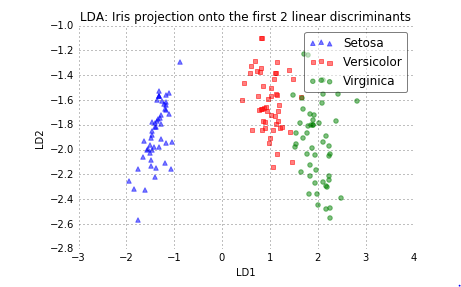
\includegraphics[scale = 1]{epp_2.PNG}
    
\end{frame}

\end{document}